\documentclass[11pt,letterpaper]{book}

%-----------------------PAQUTES---------------------------%
\usepackage{graphicx}
\usepackage[spanish]{babel}
\usepackage{float}

\usepackage{courier} %% Sets font for listing as Courier.
\usepackage{listings, xcolor}
\lstset{
tabsize = 4, %% set tab space width
showstringspaces = false, %% prevent space marking in strings, string is defined as the text that is generally printed directly to the console
numbers = left, %% display line numbers on the left
commentstyle = \color{green}, %% set comment color
keywordstyle = \color{blue}, %% set keyword color
stringstyle = \color{red}, %% set string color
rulecolor = \color{black}, %% set frame color to avoid being affected by text color
basicstyle = \small \ttfamily , %% set listing font and size
breaklines = true, %% enable line breaking
numberstyle = \tiny,
}
%\usepackage{listings}
%\usepackage{color}
%------------------------MACROS---------------------------%
%\input{sbmacros}
%-----------------------PORTADA---------------------------%
\title{Proyecto Final}
\author{Estefanía García González, Sebastián Mora Sabogal}
\begin{document}
\maketitle
\tableofcontents
\listoffigures

\part{PROYECTO}
\chapter{Caso de Estudio}
\section{Introducción}
Desde que el ser humano cuenta con raciocinio , ha buscado organizarse, desarrollar metodologías y nuevas tecnologías que faciliten su diario vivir. Ha habido un recorrido histórico en el cual las necesidades humanas de optimización de tiempo y recursos han ido en aumento, así mismo las soluciones a éstas. 
En los últimos años se ha podido apreciar una constante migración al uso de tecnologías de la información que permiten realizar a cabo tareas en todos los ámbitos de forma óptima. Uno de los actores que más se han visto inmersos en la revolución digital son los estudiantes, pero en su contexto universitario, hace falta desarrollar estrategias que le permitan mejorar la gestión de tiempo de sus actividades académicas; por lo cual se buscará una solución tecnológica que se adapte a las necesidades de los universitarios.
\section{Objetivo General}
Desarrollar un software que gestione actividades y tiempos de las asignaciones académicas a estudiantes universitarios, utilizando los modelos y metodologías de ingeniería de software para mejorar la productividad del universitario.

\section{Objetivos Específicos}
\begin{enumerate}
	\item Analizar el problema teniendo en cuenta la observación de las necesidades del estudiante, para así enfocarse en estos elementos primordiales a la hora de desarrollar el software.
	\item Presentar una solución a nivel de software a partir del previo análisis del problema para finalmente implementarlo. 
	
\end{enumerate}
\section{Descripción del problema}
La vida universitaria y académica suele ser difícil de manejar debido a la cantidad de trabajos que se deben entregar diariamente, a la prioridad que cada una es para el usuario y a la gestión de tiempo para poder realizarlos. Tareas, trabajos, talleres y grandes proyectos son algunas de las actividades que un estudiante realiza durante su semestre; además de que cada uno tiene complejidad y tiempo de realización diferentes estimados por el estudiante.
Una solución factible es la utilización de un software gestor de tareas orientado a la organización y  optimización de actividades académicas.

\section{Alcance}
Este software tendrá la capacidad de gestionar los horarios de los estudiantes, añadir recordatorios de trabajos próximos a presentar y ofrecer el servicio de organizar en horarios la realización de las tareas pendientes. Esto se llevará a cabo de acuerdo a la complejidad de la actividad a realizar, en la cual se tomará en cuenta el nivel de dificultad, si se puede desarrollar en diferentes etapas y la fecha de entrega. 

El estudiante estará en la capacidad de añadir actividades, determinar la complejidad de éstas y asignarles un horario de realización que puede ser repartido en varios bloques cuando la tarea requiere de mucho tiempo. Adicionalmente, las actividades podrán personalizarse añadiendoles objetivos a cumplir o subactividades.


\chapter{Metodología}
\section{Introducción}
La metodología del proceso de software que se debe seguir, es fundamental pues define las acciones generales que se deben llevar, a modo de conseguir un desarrollo del proyecto optimo, pasando por cada una de las fases del proceso elegido.

\section{Proceso de Software}
Parte importante de un proyecto de software es definir el, o los ciclos de vida que se manejarán dentro del proyecto, ya que estos determinarán estrategias para planificar,desarrollar y mantener el software. Por esta razón, se definirá el modelo de procesos a utilizar, tomando en cuenta los siguientes criterios:
\begin{itemize}
	\item Es necesaria una metodología que sea pertinente para un proyecto de software pequeño con pocos desarrolladores.
	\item Se considera importante la verificación en cada fase del ciclo de vida, ya que permite sentar buenas bases dentro del proyecto y reducir el riesgo.
	\item Además de la verificación, es necesaria una retroalimentación constante, ya que es posible ver con mayor claridad las falencias y carencias del proyecto.
	\item Como último criterio fundamental, se contempla la necesidad de desarrollar algunas partes de software de forma rápida, ya que esto facilitaría la retroalimentación del sistema.
\end{itemize}
Para cumplir con las pautas anteriormente mencionadas, los ciclos de vida que se elegirán son prototipo y V. Cada uno de estos modelos obedece solo a algunas de las especificaciones, pero juntos se complementan de la siguiente manera:
\begin{itemize}
	\item El modelo V es perfecto para equipos de trabajo pequeños, ya que es sencillo, de fácil aprendizaje, robusto e incluye pruebas en cada fase, lo que facilita el trabajo cuando hay pocas personas. 
	\item Gracias a los dos ciclos de vida, es posible hacer una verificación y retroalimentación de forma efectiva, ya que con el modelo en V se hacen pruebas en cada fase y con el prototipo es posible obtener resultados a corto plazo que se pueden ir revisando y evaluando.
	\item El modelo de prototipo brinda la posibilidad de construir partes del proyecto de forma prematura, por lo que es posible realizar pruebas y verificar qué cosas es necesario cambiar o añadir.
\end{itemize}
\begin{figure}
	\centering
	\includegraphics[width=0.7\linewidth]{proyecto/metodologia/imgs/Gantt}
	\caption{Cronograma. Diagrama de Gantt}
	\label{fig:gantt}
\end{figure}
\subsection{Metodología de implementación}
Los criterios que se establecieron al momento de justificar la elección los procesos de software prototipo y V, cuentan con la misma validez para determinar la metodología de implementación, debido a que para esta etapa también es necesario tener un plan de acción que beneficie la gestión de tiempos del proyecto, complemente los procesos de software, cumpliendo un proceder de forma organizada. Por esta razón se utilizará Scrum como metodología para implementar.
\begin{figure}
	\centering
	\includegraphics[width=0.7\linewidth]{proyecto/metodologia/imgs/Scrum}
	\caption{Scrum}
	\label{fig:gantt}
\end{figure}
\section{Open Source}
Desde que las personas empezaron a desarrollar software, han empezado a indagar en diferentes formas de realizar las cosas, a fin de obtener la solución computacional que solucione su necesidad. Con el tiempo estos pensamientos han devenido en ideologías que orientan la variedad de metodologías disponibles para desarrollar software.

El pensamiento o filosofía que entra en cuestión, es la del software libre, donde uno de sus principios, consiste en la reutilización del conocimiento, en este caso, el código. Es aquí donde entra el Open Source, que se relaciona con el código abierto, y con su revisión por parte de una comunidad de desarrolladores externos. Siguiendo el principio de filosofía libre, se pretende utilizar el concepto O.S con la intención de obtener una ayuda en momentos donde la implementación se torne complicada, llegandose a extrapolar a diversos casos en los que se necesite la apreciación del problema que se está trabajando por parte de un externo el cual ya lo haya desarrollado.

\part{DISEÑO}

\chapter{Requerimientos}
\section{Introducción}
Para cualquier proyecto de software, es un punto fundamental conocer cuál es la necesidad y el problema que el cliente desea resolver. Para tener una visión holística del problema, se hace necesario definir los requerimientos que satisfagan al cliente y resuelvan el problema.
\newpage

\section{Requerimientos del Cliente}
Se entiende como lo que el cliente espera encontrar cuando interactúe con la aplicación. Bajo la anterior premisa, se definieron los siguientes requerimientos:
\begin{enumerate}
	\item Añadir una tarea.
	\item Añadir subtareas para una tarea.
	\item Añadir un horario universitario.
	\item Añadir un horario de descanso (dormir).
	\item Añadir un horario de transporte.
	\item Añadir una tarea a una materia.
	\item Mostrar todas las tareas pendientes.
	\item Mostrar las tareas pendientes por materia.
	\item Mostrar las tareas pendientes por tipo.
	\item Mostrar las tareas pendientes para una fecha.
	\item Mostrar las tareas pendientes por dificultad.
	\item Mostrar el horario general del usuario.
	\item Mostrar los horarios asignados para las tareas pendientes.
	\item Modificar horario.
	\item Modificar tarea.
	\item Sugerir horarios para realizar tareas.
	\item Sugerir cuánto tiempo podría tomar una tarea.
	\item Sugerir tiempos de pausas activas durante la realización de una tarea.
	\item Alertar de la próxima entrega de una tarea.
	\item Advertir si se debe sacrificar algún espacio de descanso.

\end{enumerate}

Las siguientes tablas especificarán cada requerimiento tipo C:
 % 1.
\begin{table}[htb]
\centering
\begin{tabular}{|l|c|p{8cm}|}
\hline
RF-01 & \multicolumn {2}{p{10cm}|} {Añadir una tarea }    \\
\hline
Descripción & \multicolumn {2}{p{10cm}|} {El usuario añade una tarea pendiente por desarrollar. }\\
\hline
Precondición & \multicolumn {2}{p{10cm}|} {El usuario debe tener un horario}\\
\cline{2-3}
Secuencia & Paso & Acción \\
\cline{2-3}
& 1 & El usuario selecciona la opción de crear tarea.\\
\cline{2-3}
& 2 & El usuario proporciona la información requerida (nombre de la tarea, tipo, materia a la que pertenece) \\
& 3 & El usuario verifica la información registrada. \\
& 4 & El usuario hace selecciona el botón aceptar. \\
\hline
Postcondición & \multicolumn {2}{p{10cm}|} {El sistema muestra la tarea recién asignada con sus especificaciones y su recomendación de tiempo de realización y de horario } \\
\hline
Excepciones & Paso & Acción \\
\cline{2-3}
& 4 & Se  añade una tarea que requiere urgencia (Imprevisto). El usuario elige que horario sacrificará para realizar la tarea. \\
\cline{2-3}
& 4 & Se añade una tarea que es imposible de realizar debido al tiempo u horario. Es necesario modificar los tiempos u horarios en los que se realizará la tarea o elegir si sacrificar una frnaja de horario. \\
\hline
Rendimiento & Paso & Cota de tiempo \\
\cline{2-3}
& 1 & 1 segundo \\
\cline{2-3}
& 2 & 40 segundos \\
\cline{2-3}
& 3 & 5  segundos \\
\cline{2-3}
& 4 & 1 segundo \\
\hline
Importancia & \multicolumn {2}{p{10cm}|} {Muy importante}    \\
\hline
Urgencia & \multicolumn {2}{p{10cm}|} {urgente}    \\
\hline

\end{tabular}
\end{table}

% 2.
\begin{table}[htb]
\centering
\begin{tabular}{|l|c|p{8cm}|}
\hline
RF-02 & \multicolumn {2}{p{10cm}|} {Añadir subtareas para una tarea. }    \\
\hline
Descripcion & \multicolumn {2}{p{10cm}|} {Se añade una subtarea a una tarea.}\\
\hline
Precondición & \multicolumn {2}{p{10cm}|} {Debe existir alguna tarea pendiente.}\\
\cline{2-3}
Secuencia & Paso & Acción \\
\cline{2-3}
& 1 & El usuario selecciona la tarea a la que desea añadirle una subtarea. \\
\cline{2-3}
& 2 & Seleccionar la opción de añadir subtarea. \\
\cline{2-3}
& 3 & Se añade la subtarea como una tarea (RF-01) \\
\cline{2-3}
& 4 & El usuario verifica la información. \\
\cline{2-3}
& 5 & El pulsa la opción de aceptar. \\
\hline
Postcondición & \multicolumn {2}{p{10cm}|} {El sistema añadirá la subtarea a la tarea, mostrará sus especificaciones y recomendación de tiempo de realización y de horario} \\
\hline
Excepciones & Paso & Acción \\
\cline{2-3}
& 1 & No existe una tarea para añadirle una subtarea.  \\
\cline{2-3}
& 3 & La subtarea es de carácter urgente.
 \\
\cline{2-3}
& 4 & Se añade una subtarea y esta hace que la tarea sea imposible de terminar debido al tiempo u horario. \\

\hline
Rendimiento & Paso & Cota de tiempo \\
\cline{2-3}
& 1 & 5 segundos \\
\cline{2-3}
& 2 & 1 segundo \\
\cline{2-3}
& 3 & 40 segundos \\
\cline{2-3}
& 4 & 5 segundos  \\
\cline{2-3}
& 5 & 1 segundo \\
\hline
Importancia & \multicolumn {2}{p{10cm}|} {Importante}    \\
\hline
Urgencia & \multicolumn {2}{p{10cm}|} {No urgente}    \\
\hline
Comentarios & No. & Descripción \\
\cline{2-3}
& 1 & Añadir una subtarea es lo mismo que añadir una tarea, la deferencia es que está anidada dentro de una tarea general. \\
\hline
\end{tabular}
\end{table}

% 3.
\begin{table}[htb]
\centering
\begin{tabular}{|l|c|p{8cm}|}
\hline
RF-03 & \multicolumn {2}{p{10cm}|} {Añadir un horario universitario }    \\
\hline
Descripción & \multicolumn {2}{p{10cm}|} {Se crea un horario con materias de la universidad.}\\
\hline
Precondición & \multicolumn {2}{p{10cm}|} {Ser un usuario registrado.}\\
\cline{2-3}
Secuencia & Paso & Acción \\
\cline{2-3}
& 1 & Seleccionar la opción de crear horario. \\
\cline{2-3}
& 2 & Escribir el nombre de cada materia y su respectiva hora de inicio y fin y los días en que se repite. \\
\cline{2-3}
& 3 & El usuario añade la materia y repite el proceso cuantas veces sea necesario. \\
\cline{2-3}
& 4 & Pulsar en el botón de aceptar. \\
\hline
Postcondición & \multicolumn {2}{p{10cm}|} {El sistema guardará el horario asignado para el usuario. } \\
\hline
Excepciones & Paso & Acción \\
\cline{2-3}
& 3 & El horario de la universidad llena totalmente los espacios disponibles.
 \\
\cline{2-3}
& 3 & No hay espacios disponibles para añadir más materias al horario.
 \\
\hline
Rendimiento & Paso & Cota de tiempo \\
\cline{2-3}
& 1 & 1 segundo \\
\cline{2-3}
& 2 & 40 segundos \\
\cline{2-3}
& 3 & 2 minutos \\
\cline{2-3}
& 4 & 1 segundo \\
\hline
Importancia & \multicolumn {2}{p{10cm}|} {Muy importante}    \\
\hline
Urgencia & \multicolumn {2}{p{10cm}|} {Urgente}    \\
\hline
\end{tabular}
\end{table}

% 4.
\begin{table}[htb]
\centering
\begin{tabular}{|l|c|p{8cm}|}
\hline
RF-04 & \multicolumn {2}{p{10cm}|} {Mostrar todas las tareas pendientes. }    \\
\hline
Descripcion & \multicolumn {2}{p{10cm}|} {Se muestra la lista de tareas pendientes.}\\
\hline
Precondición & \multicolumn {2}{p{10cm}|} {Debe existir al menos una tarea pendiente.}\\
\cline{2-3}
Secuencia & Paso & Acción \\
\cline{2-3}
& 1 & Seleccionar la opción de ver las tareas pendientes. \\
\hline
Postcondición & \multicolumn {2}{p{10cm}|} {El sistema mostrará todas las tareas pendientes} \\
\hline
Excepciones & Paso & Acción \\
\cline{2-3}
& 1 & No hay tareas pendientes para mostrar.  \\
\hline
Rendimiento & Paso & Cota de tiempo \\
\cline{2-3}
& 1 & 1 segundo \\
\hline
Importancia & \multicolumn {2}{p{10cm}|} {Vital}    \\
\hline
Urgencia & \multicolumn {2}{p{10cm}|} {Urgente?}    \\
\hline
\end{tabular}
\end{table}

% 5.
\begin{table}[htb]
\centering
\begin{tabular}{|l|c|p{8cm}|}
\hline
RF-05 & \multicolumn {2}{p{10cm}|} {Mostrar el horario general del usuario. }    \\
\hline
Descripción & \multicolumn {2}{p{10cm}|} {Se muestra el horario completo del estudiante.}\\
\hline
Precondición & \multicolumn {2}{p{10cm}|} {El usuario debe haber creado un horario antes.}\\
\cline{2-3}
Secuencia & Paso & Acción \\
\cline{2-3}
& 1 & Seleccionar la opción de mostrar el horario. \\

\hline
Postcondición & \multicolumn {2}{p{10cm}|} {El sistema mostrará el horario con las materias, los descansos, los horario de transporte y las tareas pendientes} \\
\hline
Excepciones & Paso & Acción \\
\cline{2-3}
& 1 & No hay un horario para presentar.  \\

\hline
Rendimiento & Paso & Cota de tiempo \\
\cline{2-3}
& 1 & 1 segundo \\
\hline
Importancia & \multicolumn {2}{p{10cm}|} {Importante}    \\
\hline
Urgencia & \multicolumn {2}{p{10cm}|} {Puede esperar}    \\
\hline
\end{tabular}
\end{table}


% 14.
\begin{table}[htb]
\centering
\begin{tabular}{|l|c|p{8cm}|}
\hline
RF-14 & \multicolumn {2}{p{10cm}|} {Modificar horarios}    \\
\hline
Descripcion & \multicolumn {2}{p{10cm}|} {Se selecciona y modifica una franja del horario.}\\
\hline
Precondición & \multicolumn {2}{p{10cm}|} {El horario que lo que se desea modificar debe estar asignado.}\\
\cline{2-3}
Secuencia & Paso & Acción \\
\cline{2-3}
& 1 & Se selecciona la opción de modificar horario. \\
\cline{2-3}
& 2 & Se selecciona el horario de la tarea que se desea cambiar. \\
\cline{2-3}
& 3 & Se selecciona la nueva franja de horario en la que se acomodara la tarea. \\
\cline{2-3}
& 4 & El cambio de horario se ha realizado. \\
\hline
Postcondición & \multicolumn {2}{p{10cm}|} {El horario es modificado y el sistema puede ofrecer sugerencia de tiempo de realización, o incluso si se debe sacrificar algún espacio de descanso.} \\
\hline
Excepciones & Paso & Acción \\
\cline{2-3}
& 1 & No hay ningún horario para seleccionar, en este caso el caso de uso acaba.  \\
\cline{2-3}
& 3 & No existe ninguna franja disponible para cambiar, en este caso el caso de uso acaba.\\
\hline
Rendimiento & Paso & Cota de tiempo \\
\cline{2-3}
& 1 & 1 segundo \\
\cline{2-3}
& 2 & 1 segundo \\
\cline{2-3}
& 3 & 10 segundos \\
\cline{2-3}
& 4 & 1 segundo \\
\hline
Importancia & \multicolumn {2}{p{10cm}|} {Importante}    \\
\hline
Urgencia & \multicolumn {2}{p{10cm}|} {Hay presión}    \\
\hline


\end{tabular}
\end{table}

% 15.
\begin{table}[htb]
\centering
\begin{tabular}{|l|c|p{8cm}|}
\hline
RF-15 & \multicolumn {2}{p{10cm}|} {Modificar Tareas. }    \\
\hline
Descripcion & \multicolumn {2}{p{10cm}|} {Se permite modificar los diferentes campos de una tarea.}\\
\hline
Precondición & \multicolumn {2}{p{10cm}|} {Debe existir alguna tarea para modificar.}\\
\cline{2-3}
Secuencia & Paso & Acción \\
\cline{2-3}
& 1 & Se solicita modificar una tarea. \\
\cline{2-3}
& 2 & El usuario selecciona la tarea que desea modificar. \\
\cline{2-3}
& 3 & El usuario selecciona el campo de la tarea que desea modificar. \\
\cline{2-3}
& 4 & Se modifica el campo de la tarea. \\
\cline{2-3}
& 5 & Se permite elegir realizar otro cambio o terminar. \\
\hline
Postcondición & \multicolumn {2}{p{10cm}|} {La tarea tiene un campo modificado, según el tipo podría haber una sugerencia, como en el caso de dificultad, o cambio de horario para realizarse.} \\
\hline
Excepciones & Paso & Acción \\
\cline{2-3}
& 3 & Si la tarea solo tiene los campos minimos se puede agregar el cambio, así el caso de uso continua.   \\
\hline
Rendimiento & Paso & Cota de tiempo \\
\cline{2-3}
& 1 & 1 segundo \\
\cline{2-3}
& 2 & 1 segundo \\
\cline{2-3}
& 3 & 1 segundo \\
\cline{2-3}
& 4 & 5 segundos \\
\cline{2-3}
& 5 & 1 segundo \\
\hline
Importancia & \multicolumn {2}{p{10cm}|} {vital}    \\
\hline
Urgencia & \multicolumn {2}{p{10cm}|} {Hay presión}    \\
\hline
\end{tabular}
\end{table}

% 16.
\begin{table}[htb]
\centering
\begin{tabular}{|l|c|p{8cm}|}
\hline
RF-16 & \multicolumn {2}{p{10cm}|} {Sugerir horarios para realizar tareas.}    \\
\hline
Descripcion & \multicolumn {2}{p{10cm}|} {Según los horarios disponibles, al momentos de adicionar una tarea se hace una sugerencia de horario para realizarla.}\\
\hline
Precondición & \multicolumn {2}{p{10cm}|} {Se debe haber agregado una tarea, y deben haber horarios disponibles para hacer la recomendación.}\\
\cline{2-3}
Secuencia & Paso & Acción \\
\cline{2-3}
& 1 & Al momento de agregar una tarea, se revisan horarios disponibles. \\
\cline{2-3}
& 2 & Se revisan las variables de la tarea (dificultad, fecha de entrega). \\
\cline{2-3}
& 3 & Se hace la recomendación. \\
\hline
Postcondición & \multicolumn {2}{p{10cm}|} {La recomendación se dará al usuario dandole la posibilidad de tomarla o dejarla.} \\
\hline
Excepciones & Paso & Acción \\
\cline{2-3}
& 1 & Puede pasar que no haya horarios disponibles para hacer la recomendación, así el caso de uso termina.  \\
\cline{2-3}
& 2 & Si no hay variables de tarea definidos, se pasa al siguiente paso. \\
\hline
Rendimiento & Paso & Cota de tiempo \\
\cline{2-3}
& 1 & 5 segundos \\
\cline{2-3}
& 2 & 5 segundos \\
\cline{2-3}
& 2 & 1 segundo \\
\hline
Importancia & \multicolumn {2}{p{10cm}|} {Normal}    \\
\hline
Urgencia & \multicolumn {2}{p{10cm}|} {Puede esperar}    \\
\hline
Comentarios & No. & Descripción \\
\cline{2-3}
& 1 & El caso de uso esta bastante ligado a otros casos de uso, como puede apreciarse en el diagrama, sin embargo su relevancia no es la misma como la de los casos a los que apoya. \\
\hline
\end{tabular}
\end{table}

% 19.
\begin{table}[htb]
\centering
\begin{tabular}{|l|c|p{8cm}|}
\hline
RF-19 & \multicolumn {2}{p{10cm}|} {Alertar de la próxima entrega de una tarea. }    \\
\hline
Descripcion & \multicolumn {2}{p{10cm}|} {Se pretende avisar con tiempo prudencial que el ciclo de una tarea esta por finalizar, lo cual significa que debe ser terminada para ser entregada.}\\
\hline
Precondición & \multicolumn {2}{p{10cm}|} {La existencia de la tarea.}\\
\cline{2-3}
Secuencia & Paso & Acción \\
\cline{2-3}
& 1 & Se revisa el tiempo para que la tarea deba ser terminada comparandolo con el prudencial. \\
\cline{2-3}
& 2 & Se realiza el aviso. \\
\hline
Postcondición & \multicolumn {2}{p{10cm}|} {El usuario será avisado sobre la proximidad de su tarea.} \\
\hline
Excepciones & Paso & Acción \\
\cline{2-3}
& 1 & Si la tarea no cuenta con tiempo de realización se considera indefinida, así el caso de uso termina.  \\
\hline
Rendimiento & Paso & Cota de tiempo \\
\cline{2-3}
& 1 & 1 segundo \\
\cline{2-3}
& 2 & 1 segundo \\
\hline
Importancia & \multicolumn {2}{p{10cm}|} {Importante}    \\
\hline
Urgencia & \multicolumn {2}{p{10cm}|} {Puede esperar}    \\

\hline
\end{tabular}
\end{table}




\include{diseno/interaccion/interaccion}
\chapter{Clases}
\section{Introducción}
Los diagramas de clase son parte importante del diseño de un software, ya que estos permiten generar diseños que plasmen la solución a un problema, la cual será entendible para todos aquellos conozan del lenguaje unificado de modelado (UML).
\\
Además es necesario utilizar diagramas de clase para representar gráficamente y de forma estática la estructura general del sistema, mostrando sus clases e interacciones.
\section{Teoría}
Los diagramas de clase sirven para visualizar las relaciones entre las clases que involucran el sistema,entre estas se encuentran:
\begin{itemize}
\item Dependencia.
\item Asociación.
\item Agregación.
\item Composición.
\item Generalización.
\item Realización.
\end{itemize}

Estas relaciones pueden subdividirse en dos grandes grupos: Las relaciones cliente/proveedor, en las cuales entran las dependencias y asociaciones (asociación, agregación y composición), las cuales generan un alto acoplamiento en el software, pero también lo hacen seguro. Por otro lado están las relaciones de generalizacion en las cuales están la especialización e implementacion. Estas poseen un bajo acoplamiento, pero no poseen la seguridad de las de cliente/proveedor. 
El ideal es crear un diagrama de clases en el que haya un equilibrio entre el acoplamiento y la seguridad.
\begin{figure}[H]
	\centering
	\includegraphics[width=1\linewidth]{diseno/clases/imagenes/relaciones.png}
	\caption{Relaciones UML. Tomada de internet}
	\label{fig:gantt}
\end{figure}
Por otro lado, las clases se representan por medio de un rectángulo que se divide en tres:
\begin{itemize}
\item Nombre de la clase: Cómo se denomina la clase. Es un sustantivo.
\item Atributos de la clase: Pueden ser de diferentes tipos (booleano, numérico, cadenas Y T.D.A), tienen modificadores de visibilidad (public, private, protected, de paquete), nombre y propiedades (final, const) si es necesario.
\item Métodos de la clase: Son las operaciones que realiza la clase, deben denominarse con verbos, poseen modificadores de visibilidad y pueden retornar diferentes tipos de datos (void, numérico, cadenas y T.D.A) Adicionalmente, los métodos pueden recibir argumentos, que se representan en las operaciones en forma de parámetros los cuales son variables que poseen nombre y tipo.
\end{itemize}
 
\chapter{Patrones}
\section{Introducción}
Aunque históricamente el software pueda considerarse como primitivo si se compara con otras disciplinas que llevan siglos de ventaja en cuanto a su desarrollo, actualmente no es así. La anterior reflexión se deduce debido a que el software ha evolucionado lo suficiente para convertirse en una herramienta que va mas allá de solo programar, también se encarga de diseñar y modelar. En este caso, el diseño de software puede generar soluciones generalizadas a problemas reincidentes. Así es como llegamos a los patrones de diseño, los cuales para cualquier proyecto, independientemente de su complejidad y tamaño, seguramente se verán involucrados.

A partir de lo anterior, es claro que los patrones de diseño aparecerán en la propuesta de estructura del proyeto, más conocida como diagrama de clases, con la intención de obtener un diagrama razonable desde un punto de vista de principios de diseño así como los principios del paradigma orientado a objetos. 

Se debe mencionar también que los patrones propuestos en este documento, no necesariamente todos están incluidos en el Gof (the Gang of Four), pues existen otras soluciones que aunque no tan conocidas, pueden tener un impacto positivo debido en el desarrollo del software.
\newpage

\section{Patrón Composite}
El patrón de diseño Composite (Componente), nos permite construir estructuras complejas partiendo de otras estructuras mucho mas simples, lo cual permite crear estructuras compuestas conformadas por otras mas pequeñas. Este patrón resulta útil para la creación de subtareas dentro de una tarea mas general, ya que se genera una estructura en forma de árbol gracias a la recursividad con la que funciona el patrón. Otra ventaja de su utilización, en este desarrollo específicamente,  es que se puede representar la jerarquía de tarea-subtarea, además de añadir dinamismo a la tarea, ya que ésta puede tener subtareas de diferentes tipos. Además es posible tratar la subtarea como tarea.
\\
En conclusión, el patrón componente posibilita la solución del problema de las subtareas, ya que permite jerarquizar, añadir dinamismo a la tarea por medio de subtareas y construir la tarea general por medio de subtareas, por esta razón será utilizado dentro de este software.

\begin{figure}[H]
	\centering
	\includegraphics[width=1\linewidth]{diseno/patrones/imgs/Composite}
	\caption{Patrón Componente}
	\label{fig:gantt}
\end{figure}

\section{Patrón agrupador}
Un horario puede mostrarse como la constitución de diversas franjas en un orden lógico; estas deben agruparse para que haya orden y se puedan manejar conjuntamente. Por está razón el patrón agrupación será de utilidad, ya que permite generar una estructura en la cual los módulos, que en este caso son las franjas, puedan ser agrupados para invocarse de forma colectiva como el horario, de esta forma se centraliza el control de la estructura en una sola clase.

\begin{figure}[H]
	\centering
	\includegraphics[width=0.5\linewidth]{diseno/patrones/imgs/Agrupador}
	\caption{Patrón Agrupador}
	\label{fig:gantt}
\end{figure}

\section{Patrón Fábrica Abstracta}
La creación de objetos es una situación que aparece en prácticamente cualquier proyecto, por lo que se debe buscar una estructura que permita llevar esta creación de la mejor manera, incluso en mayor medida cuando el objeto a crear pertenece a una familia de otros objetos que también pueden ser creados, y por supuesto en un caso más general en caso de que hayan varias de estas familias de objetos.

La fábrica abstracta lo que hace es esto, proveer una interfaz para la creación de estas familias de objetos relacionados, sin especificar sus clases concretas.

Para el caso del proyecto, la fábrica abstracta es útil pues existen dos familias de objetos a crear, una de tareas referente a lo académico y otra la de tareas que no tienen que ver con la universidad.

\begin{figure}[H]
	\centering
	\includegraphics[width=1\linewidth]{diseno/patrones/imgs/FabricaAbstracta}
	\caption{Patrón Fábrica Abstracta}
	\label{fig:gantt}
\end{figure}

\section{Patrón Estrategia}
Dada la situación de que un programa pueda ofrecer un servicio, el cual se pueda realizar de varias maneras hace alusión a este patrón. La intención de este es poder seleccionar la alternativa más adecuada para el cliente, durante tiempo de ejecución.

En la mención a la fábrica abstracta se mencionaron las familias de objetos de tarea y categoria, las cuales en algún momento necesitarán de la posibilidad de una modificación de alguno de sus objetos, operación que no solo involucra a este último en cuestión, sino que abarca principalmente el modulo externo de manejo de base de datos. Dependiendo de cada objeto, la misma operación debe hacerce de manera distinta, haciendo así que entre el patrón estrategia.

\begin{figure}[H]
	\centering
	\includegraphics[width=1\linewidth]{diseno/patrones/imgs/Estrategia}
	\caption{Patrón Estrategia}
	\label{fig:gantt}
\end{figure}

\chapter{Estados}
\section{Introducción}
A medida que se realiza una solución a un problema, los objetos deberán interactuar para llegar a esta solución, y en medio de esas interacciones, habrán acciones que incentiven el cambio de estado de uno o varios de esos objetos
\newpage
\section{Marco Teórico}

\section{Diagramas de estado}
Abarcando el problema que se esta resolviendo, se determinó que el objeto al cual se le deben aclarar sus estados, es el de tarea, pues hace parte fundamental en la solución del problema, así que el entendimiento de sus estados a lo largo de la ejecución del software que pretende implementarla será crucial.

\begin{figure}[H]
	\centering
	\includegraphics[width=1\linewidth]{diseno/estados/imgs/estadosTarea}
	\caption{Diagrama de estados para el objeto Tarea.}
	\label{fig:gantt}
\end{figure}

Cabe mencionar, de manera obligatoria, que este diagrama tendrá su correspondiente planeación estructural, que en otras palabras vendría a ser su espacio en el diagrama de clases de toda la solución. Para esto, existe un patrón de comportamiento, que precisamente tiene como objetivo cumplir el principio de diseño abierto/cerrado en el contexto de estados de un objeto.

\begin{figure}[H]
	\centering
	\includegraphics[width=1\linewidth]{diseno/estados/imgs/PatronState}
	\caption{Patrón state para solucionar los estados del objeto Tarea.}
	\label{fig:gantt}
\end{figure}

\begin{figure}[H]
	\centering
	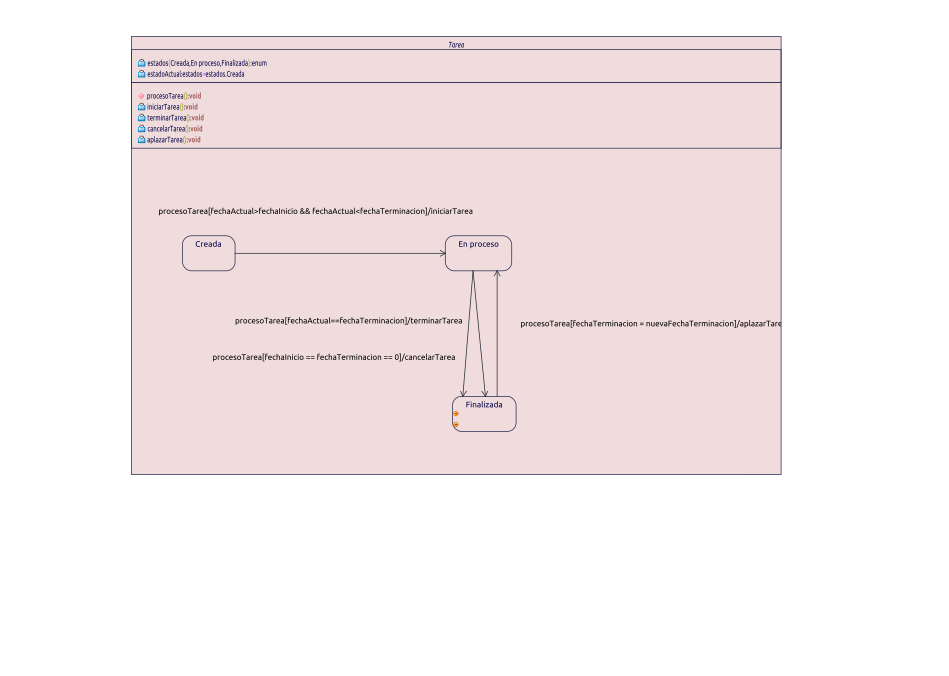
\includegraphics[width=1\linewidth]{diseno/estados/imgs/loquesea.pdf}
	\caption{Detalle de la clase Tarea bajo el contexto del patrón Estado.}
	\label{fig:gantt}
\end{figure}
\chapter{Componentes}
\section{Introducción}
Por lo general, un proyecto de software está compuesto por diferentes funcionalidades, las cuales al juntarse, proveen lo que deseamos que el software realice. Adicionalmente, esas funcionalidades pueden ser usadas individualmente e incluso en otros proyectos. Cada una de ellas se recoge en lo que llamamos componente. Estos elementos se comportan como una caja negra, ya que realizan su función, pero sin mostrar cómo lo hacen internamente. Esto trae ventajas tanto de seguridad, por el encapsulamiento, como de facilidad de uso por las interfaces que provee o solicita.
Por esta razón, la utilización de componentes es ventajosa para realizar este proyecto de software, ya que se generarán componentes independientes que puedan ser reutilizados en un futuro y además, la dependencia entre ellos será baja ya que se gestionarán entre interfaces.
\section{Diagrama de componentes}
\begin{figure}[H]
	\centering
	\includegraphics[width=1\linewidth]{diseno/componentes/img/diagramaComponentes}
	\caption{Diagrama de componentes}
	\label{fig:componentes}
\end{figure}
Las funcionalidades de los componentes del diagrama son:
\begin{itemize}
	\item Interfaz gráfica: Este componente le ofrece una interfaz gráfica al software, sólo se comunica con el gestorPrincipal para solicitarle la información que necesita mostrar.
	\item Agenda: La agenda organiza las tareas de acuerdo al horario, por lo tanto se comunica con ambos componentes para solicitar la información que necesita para realizar su tarea. Luego le envía la información al componente de interfaz gráfica, para que muestre la información.
	\item Horario: Realiza todas las funciones como crear, modificar, ordenar el horario del estudiante. Se comunica con la persistencia para solicitar información.
	\item Tarea: Se encarga de realizar funciones como crear y  modificar tareas. Se comunica con la persistencia para obtener la información que necesita.
	\item Persistencia: Es el componente que se comunica con la base de datos y brinda fachadas para que los componentes que lo necesiten hagan consultas o ingresen información en la vase de datos.
\end{itemize}
	

\chapter{Nodos}
\section{Introducción}
Un diagrama de nodos o de despliegue muestra las relaciones físicas de los nodos que la componen, además de cómo se reparten los nodos en cada nodo. Algunas de las ventajas de el uso de este tipo  de diagramas es la visión holística que se puede tener del proyecto, ya que muestra la relación y distribución de la parte de hardware y software. El problema de esto es que al ser tan general no se pueden vislumbrar algunos detalles que si se pueden ver en otro tipo de diagramas.
\section{Marco Teórico}
Un diagrama de despliegue se compone de:
\begin{itemize}
\item Nodo: Es un elemento de hardware o software que se muestra como una caja en tres dimensiones.
\begin{figure}[H]
	\centering
	\includegraphics[width=0.5\linewidth]{diseno/nodos/imgs/1}
	\caption{Nodo. Imagen tomada de internet}
	\label{fig:gantt}
\end{figure}

\item Instancia de nodo: Una instancia se puede distinguir de un nodo por el hecho de que su nombre esta subrayado y tiene dos puntos antes del tipo de nodo base. 
\begin{figure}[H]
	\centering
	\includegraphics[width=0.5\linewidth]{diseno/nodos/imgs/2}
	\caption{Instancia de un nodo. Imagen tomada de internet}
	\label{fig:gantt}
\end{figure}

\item Estereotipo de nodo: Estereotipos estándar se proveen para los nodos, nombrados «cdrom», «cd-rom», «computer», «disk array», «pc», «pc client», «pc server», «secure», «server», «storage», «unix server», «user pc». Estos mostrarán un icono apropiado en la esquina derecha arriba del símbolo nodo.

\begin{figure}[H]
	\centering
	\includegraphics[width=0.7\linewidth]{diseno/nodos/imgs/3}
	\caption{Estereotipo de Nodo. Imagen tomada de internet}
	\label{fig:gantt}
\end{figure}

\item Artefacto: Un artefacto es un producto del proceso de desarrollo de software, que puede incluir los modelos del proceso como los casos de uso, los modelos de diseño, etc.

\begin{figure}[H]
	\centering
	\includegraphics[width=0.5\linewidth]{diseno/nodos/imgs/4}
	\caption{Artefacto. Imagen tomada de internet}
	\label{fig:gantt}
\end{figure}

\end{itemize}

\section{Diagrama de nodos}
\begin{figure}[H]
	\centering
	\includegraphics[width=0.8\linewidth]{diseno/nodos/imgs/nodos}
	\caption{Artefacto. Imagen tomada de internet}
	\label{fig:gantt}
\end{figure}

\chapter{Actividades}
\section{Introducción}
Los diagramas de actividades, junto a los de clases y casos de uso, son diagramas de comportamiento, ya que describen como funcionará ya sea de un algoritmo o incluso de un componente completo. Estos brindan grandes ventajas, como lo es mostrar un flujo de trabajo entre los usuarios y un sistema, clarificar ese tipo de procesos y traer simplificación.
Por ello, para describir cómo será el flujo de trabajo del software, se utilizarán los diagramas de actividades ya que estos permiten detallar en un lenguaje de alto nivel, los procesos que se llevan a cabo. 
\section{Marco Teórico}
Un diagrama de actividades está constituido por:
\begin{itemize}
\item Actividad: Es un comportamiento que describe una serie de acciones de forma determinada y organizada.
\begin{figure}[H]
	\centering
	\includegraphics[width=0.5\linewidth]{diseno/actividades/imgs/1}
	\caption{Actividad. Imagen tomada de internet}
	\label{fig:gantt}
\end{figure}
\item Acción: Una acción representa un solo paso dentro de una actividad. Las acciones se denotan por rectángulos con las puntas redondeadas.
\begin{figure}[H]
	\centering
	\includegraphics[width=0.5\linewidth]{diseno/actividades/imgs/3}
	\caption{Accion. Imagen tomada de internet}
	\label{fig:gantt}
\end{figure}
\item Flujo de control: Este muestra el flujo de una acción a otra. Se denota por una flecha.
\begin{figure}[H]
	\centering
	\includegraphics[width=0.5\linewidth]{diseno/actividades/imgs/2}
	\caption{Flujo de control. Imagen tomada de internet}
	\label{fig:gantt}
\end{figure}
\item Nodo inicial: Es el primer nodo, se describe por un gran punto negro.
\begin{figure}[H]
	\centering
	\includegraphics[width=0.5\linewidth]{diseno/actividades/imgs/6}
	\caption{Nodo inicial. Imagen tomada de internet}
	\label{fig:gantt}
\end{figure}
\item Nodo de decisión y combinación: Los nodos de decisión y combinación tienen la misma notación: una forma de diamante.  Los flujos de control que provienen de un nodo de decisión tendrán condiciones de guarda que permitirán el control para fluir si la condición de guarda se realiza.
\begin{figure}[H]
	\centering
	\includegraphics[width=0.5\linewidth]{diseno/actividades/imgs/4}
	\caption{Nodo de decisión y combinación. Imagen tomada de internet}
	\label{fig:gantt}
\end{figure}
\item Nodo de bifurcación y unión: Las bifurcaciones y uniones tienen la misma notación: una barra a la que llegan o de la que salen flujos de control). Estos indican el comienzo y final de hilos actuales de control.
\begin{figure}[H]
	\centering
	\includegraphics[width=0.5\linewidth]{diseno/actividades/imgs/5}
	\caption{Nodo de bifurcación y unión. Imagen tomada de internet}
	\label{fig:gantt}
\end{figure}
\item Particiones: 	Una partición se utiliza para separar acciones dentro de una actividad, se denota de la siguiente manera:
\begin{figure}[H]
	\centering
	\includegraphics[width=0.5\linewidth]{diseno/actividades/imgs/7}
	\caption{Partición. Imagen tomada de internet}
	\label{fig:gantt}
\end{figure}
\end{itemize}
%http://www.sparxsystems.com.ar/resources/tutorial/uml2_activitydiagram.html
\section{Diagrama de actividades}
\begin{figure}[H]
	\centering
	\includegraphics[width=1\linewidth]{diseno/actividades/imgs/actividades}
	\caption{Diagrama de actividades. Fuente autor.}
	\label{fig:gantt}
\end{figure}
\part{REFLEXIONES}
k\chapter{Conclusiones}

\begin{itemize}
\item Luego de haber pasado por las diferentes etapas del proceso de ingenieria de softaware, se empieza a formar la noción del porqué existen estas prácticas, cuestión que va de la mano teniendo en cuenta el contexto, en el sentido de que el problema que se abordo, contempla una mayor magnitud, y aún en caso contrario, se hubiese podido dar el mismo tratamiento.

\item Entrando en contexto con las prácticas en sí, el proceso que las reúne, conlleva la idea de la planificación, término que en principio, no se entiende la concepción que posee en el contexto del software, sin embargo, es una idea que toma forma a medida que se realizan las etapas. Tanto es así, que en el momento de ejecutar cada etapa, en varias ocasiones fue necesario volver a una etapa anterior, revisar, y adaptar, síntoma claro de falta de visión al momento de ejecutar el análisis. Sin embargo cabe destacar que fue algo necesario, e incluso esperado al ser la primera vez en ejecutar un proceso de ingeniería de software.

\item Al ser el software en cuestión enfocado hacia los estudiantes, la concepción del problema basado en las necesidades que tendría un estudiante para manejar sus tiempos, no fue complicada, más bien las ideas plasmadas se orientan bastante en las necesidades generalizadas. El abarcar necesidades más específicas, no fue tenido en cuenta, pues hubiese supuesto una mayor complejidad, que viendo los tiempos disponibles para implementar el proyecto, no sería factible. 
\end{itemize}


\newpage
%---bibliografia
\bibliographystyle{plain}
\bibliography{}

\end{document}